\subsection{Conversion from Depth-Image to Feature Image}

For transition from depth-based to feature-based registration a prior conversion from depth values to a derived image is required.
Every feature-image is calculated on range data in floating point format.
Conversion from integer data does no further processing then simply type conversion.

\subsubsection{\Glspl{bearing-angle-image}}

\begin{figure}[H]
    \centering
    

\tikzset{every picture/.style={line width=0.75pt}} %set default line width to 0.75pt        

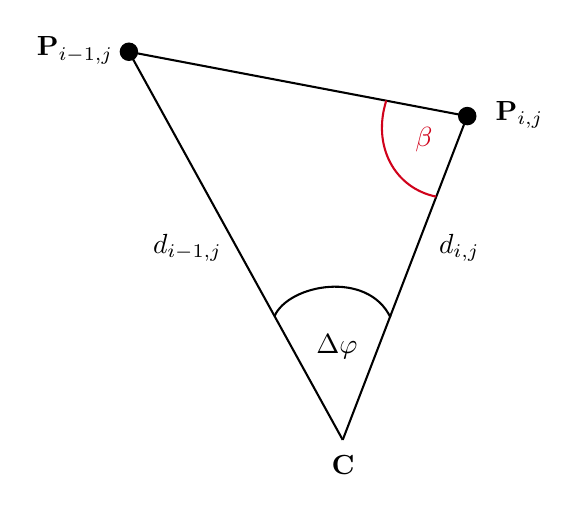
\begin{tikzpicture}[x=0.75pt,y=0.75pt,yscale=-1,xscale=1]
%uncomment if require: \path (0,228); %set diagram left start at 0, and has height of 228

%Straight Lines [id:da05017383740499093] 
\draw    (42.83,15.67) -- (145.83,202.67) ;
%Straight Lines [id:da6895513561877372] 
\draw    (205.83,46.67) -- (145.83,202.67) ;
%Curve Lines [id:da10253757735662583] 
\draw [color={rgb, 255:red, 0; green, 0; blue, 0 }  ,draw opacity=1 ]   (113,143) .. controls (119.83,127.67) and (157.83,120.67) .. (168.83,143.67) ;
%Straight Lines [id:da3851492122035306] 
\draw    (42.83,15.67) -- (205.83,46.67) ;
%Curve Lines [id:da7052636563383052] 
\draw [color={rgb, 255:red, 208; green, 2; blue, 27 }  ,draw opacity=1 ]   (166.83,39.17) .. controls (159.83,61.17) and (170.9,81.48) .. (190.9,85.48) ;
%Shape: Circle [id:dp08101382020617043] 
\draw  [fill={rgb, 255:red, 0; green, 0; blue, 0 }  ,fill opacity=1 ] (201.88,46.67) .. controls (201.88,44.49) and (203.65,42.72) .. (205.83,42.72) .. controls (208.01,42.72) and (209.78,44.49) .. (209.78,46.67) .. controls (209.78,48.85) and (208.01,50.62) .. (205.83,50.62) .. controls (203.65,50.62) and (201.88,48.85) .. (201.88,46.67) -- cycle ;
%Shape: Circle [id:dp7397482298206297] 
\draw  [fill={rgb, 255:red, 0; green, 0; blue, 0 }  ,fill opacity=1 ] (38.88,15.67) .. controls (38.88,13.49) and (40.65,11.72) .. (42.83,11.72) .. controls (45.01,11.72) and (46.78,13.49) .. (46.78,15.67) .. controls (46.78,17.85) and (45.01,19.62) .. (42.83,19.62) .. controls (40.65,19.62) and (38.88,17.85) .. (38.88,15.67) -- cycle ;

% Text Node
\draw (143,158) node  [color={rgb, 255:red, 0; green, 0; blue, 0 }  ,opacity=1 ] [align=left] {$\displaystyle \Delta $$\displaystyle \varphi $};
% Text Node
\draw (185,58) node  [color={rgb, 255:red, 208; green, 2; blue, 27 }  ,opacity=1 ] [align=left] {$\displaystyle \beta $};
% Text Node
\draw (202,110) node   [align=left] {$\displaystyle d_{i,j}$};
% Text Node
\draw (71,110) node   [align=left] {$\displaystyle d_{i-1,j}$};
% Text Node
\draw (231,46) node   [align=left] {$\displaystyle \mathbf{P}_{i,j}$};
% Text Node
\draw (16.83,15) node   [align=left] {$\displaystyle \mathbf{P}_{i-1,j}$};
% Text Node
\draw (146,215) node   [align=left] {$\displaystyle \mathbf{C}$};


\end{tikzpicture}

%
    \caption[Schematic Representation of Bearing-Angles]{This figure shows the relationship of the light rays that form the \gls{bearing-angle}.}
\end{figure}

Existing literature\cite{Scaramuzza2007,Lin2017} proposes \Glspl{bearing-angle-image} were each pixel is the angle between the current point, the optical center and the previous point.
The neighbourhood relationship can be choosen arbitrarily resulting in four first-order \Glspl{bearing-angle-image}, horizontal, vertical, diagonal and antidiagonal.
The second variable is the direction the angle is calculted, e.g.~for horizontal images it can be calculated from left-to-right or right-to-left.
This does not exhibit new information, because the angle of the other direction is immediatly known from the fact that the sum of the angles is $180\degree$.
Nontheless, the direction must be defined to obtain stable visual features.

The formula for the \gls{bearing-angle} $\beta$ is derived with the cosine theorem.
For the horizontal left-to-right calculation the formula is as follows.
\begin{equation}
    \beta = \arccos%
            \frac{d_{i,j} - d_{i-1,j} \cos \Delta\varphi}%
                 {\sqrt{d_{i,j}^2 + d_{i-1,j}^2 - 2 d_{i,j} d_{i-1,j} \cos \Delta\varphi}}
\end{equation}
Using a different direction or other neighbourhood relation the indices for the depth values need to be changed and a different angular resolution needs to be calculated.
The \Gls{bearing-angle} is in the range $\beta \in (0, \pi)~rad$.
Linear scaling of the angle to the color depth of the target image results in a grayscale image suitable for feature extraction.
A general scaling function for an $unsigned~8bit$ image and arbitrary angle range follows here.
This formulation can be used for different color depths and other potential angle calculations that result in different boundary conditions.
\begin{equation}
\begin{aligned}
    \beta_{min} &= 0 ~& c_{min} &= 0 \\
    \beta_{max} &= \pi ~& c_{max} &= 255 \\
    \beta_{scaled} &= \floor*{c_{min} + \beta \frac{c_{max} - c_{min}}{\beta_{max} - \beta_{min}}}
\end{aligned}
\end{equation}

\subsubsection{\Glspl{flexion-image}}\label{flexion-image-section}

Each pixel of a \Gls{flexion-image} is the dot-product of the local normal
calculated from horizontal and vertical neighbouring pixel with the
normal calculated with the diagonal neighbours.
Figure~\ref{fig:flexion-image-scetched} demonstrates the disparity of both normals for an arbitrary surface patch.
The normal calculated from the diagonal and vertical neighbouring vertices are drawn in blue and the normal calculated with the diagonals red.
Both normal-vectors are drawn with their origin in the central depth value.

\begin{figure}[H]
    \begin{subfigure}[t]{0.49\linewidth}
        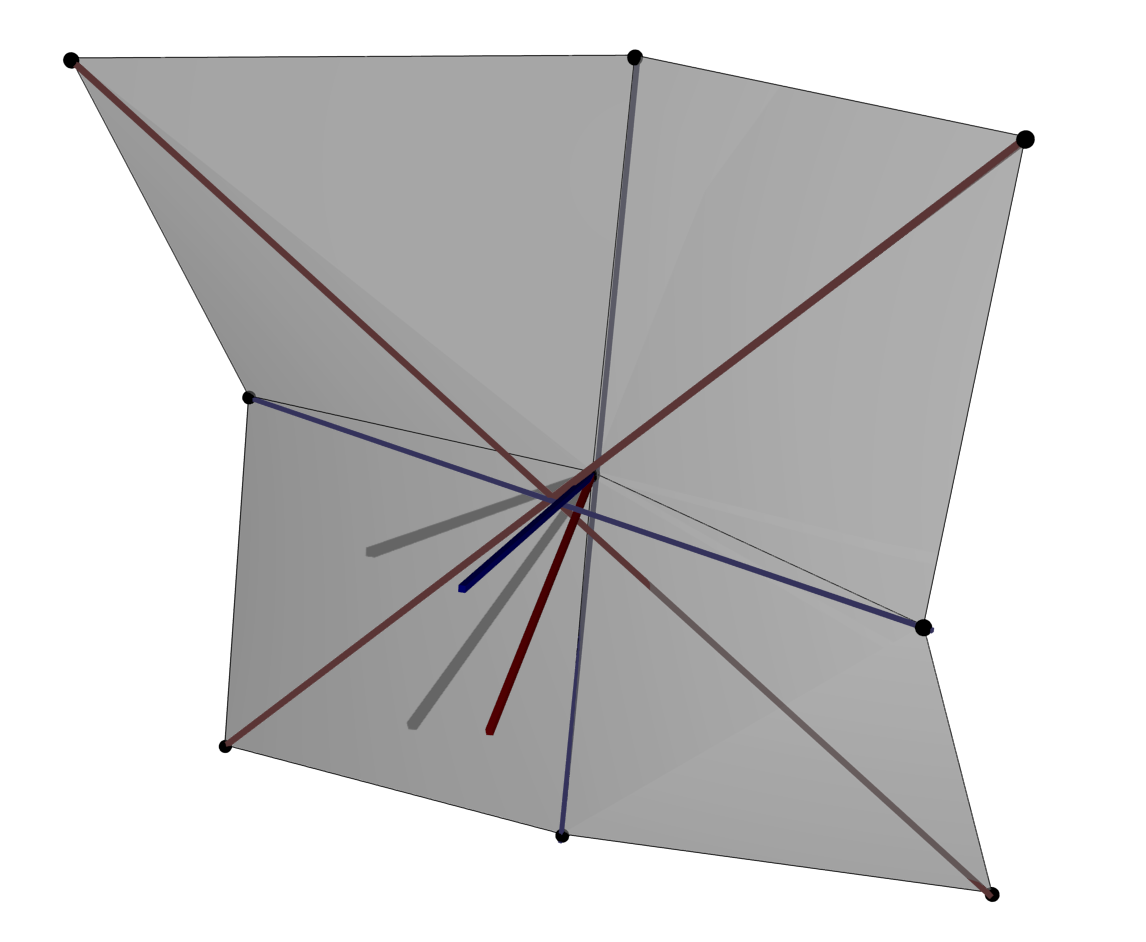
\includegraphics[width=0.9\textwidth]{chapter04/img/scetch_flexion.png}
    \end{subfigure}
    \begin{subfigure}[t]{0.49\linewidth}
        

\tikzset{every picture/.style={line width=0.75pt}} %set default line width to 0.75pt        

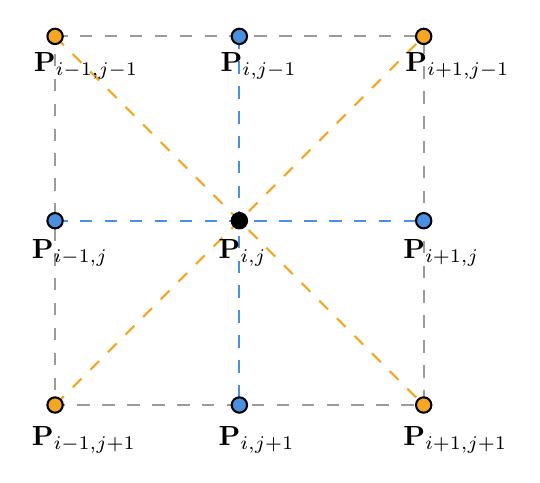
\begin{tikzpicture}[x=0.75pt,y=0.75pt,yscale=-1,xscale=1]
%uncomment if require: \path (0,237); %set diagram left start at 0, and has height of 237

%Shape: Rectangle [id:dp6565487036659107] 
\draw  [color={rgb, 255:red, 155; green, 155; blue, 155 }  ,draw opacity=1 ][dash pattern={on 4.5pt off 4.5pt}] (28.7,13.7) -- (206.3,13.7) -- (206.3,191.3) -- (28.7,191.3) -- cycle ;
%Straight Lines [id:da30195081571029425] 
\draw [color={rgb, 255:red, 74; green, 144; blue, 226 }  ,draw opacity=1 ] [dash pattern={on 4.5pt off 4.5pt}]  (28.7,102.5) -- (206.3,102.5) ;
%Straight Lines [id:da4586174781414081] 
\draw [color={rgb, 255:red, 74; green, 144; blue, 226 }  ,draw opacity=1 ] [dash pattern={on 4.5pt off 4.5pt}]  (117.5,13.7) -- (117.5,191.3) ;
%Straight Lines [id:da7294828306266232] 
\draw [color={rgb, 255:red, 245; green, 166; blue, 35 }  ,draw opacity=1 ] [dash pattern={on 4.5pt off 4.5pt}]  (28.7,13.7) -- (206.3,191.3) ;
%Straight Lines [id:da3243995266948473] 
\draw [color={rgb, 255:red, 245; green, 166; blue, 35 }  ,draw opacity=1 ] [dash pattern={on 4.5pt off 4.5pt}]  (28.7,191.3) -- (206.3,13.7) ;
%Shape: Circle [id:dp5266363779447065] 
\draw  [fill={rgb, 255:red, 245; green, 166; blue, 35 }  ,fill opacity=1 ] (25,13.7) .. controls (25,11.66) and (26.66,10) .. (28.7,10) .. controls (30.74,10) and (32.4,11.66) .. (32.4,13.7) .. controls (32.4,15.74) and (30.74,17.4) .. (28.7,17.4) .. controls (26.66,17.4) and (25,15.74) .. (25,13.7) -- cycle ;
%Shape: Ellipse [id:dp14497174740803043] 
\draw  [fill={rgb, 255:red, 74; green, 144; blue, 226 }  ,fill opacity=1 ] (25,102.5) .. controls (25,100.46) and (26.66,98.8) .. (28.7,98.8) .. controls (30.74,98.8) and (32.4,100.46) .. (32.4,102.5) .. controls (32.4,104.54) and (30.74,106.2) .. (28.7,106.2) .. controls (26.66,106.2) and (25,104.54) .. (25,102.5) -- cycle ;
%Shape: Ellipse [id:dp0427609892023727] 
\draw  [fill={rgb, 255:red, 245; green, 166; blue, 35 }  ,fill opacity=1 ] (25,191.3) .. controls (25,189.26) and (26.66,187.6) .. (28.7,187.6) .. controls (30.74,187.6) and (32.4,189.26) .. (32.4,191.3) .. controls (32.4,193.34) and (30.74,195) .. (28.7,195) .. controls (26.66,195) and (25,193.34) .. (25,191.3) -- cycle ;
%Shape: Ellipse [id:dp2872052196845898] 
\draw  [fill={rgb, 255:red, 74; green, 144; blue, 226 }  ,fill opacity=1 ] (113.8,13.7) .. controls (113.8,11.66) and (115.46,10) .. (117.5,10) .. controls (119.54,10) and (121.2,11.66) .. (121.2,13.7) .. controls (121.2,15.74) and (119.54,17.4) .. (117.5,17.4) .. controls (115.46,17.4) and (113.8,15.74) .. (113.8,13.7) -- cycle ;
%Shape: Circle [id:dp758793708555806] 
\draw  [fill={rgb, 255:red, 0; green, 0; blue, 0 }  ,fill opacity=1 ] (113.8,102.5) .. controls (113.8,100.46) and (115.46,98.8) .. (117.5,98.8) .. controls (119.54,98.8) and (121.2,100.46) .. (121.2,102.5) .. controls (121.2,104.54) and (119.54,106.2) .. (117.5,106.2) .. controls (115.46,106.2) and (113.8,104.54) .. (113.8,102.5) -- cycle ;
%Shape: Circle [id:dp477059334030714] 
\draw  [fill={rgb, 255:red, 74; green, 144; blue, 226 }  ,fill opacity=1 ] (113.8,191.3) .. controls (113.8,189.26) and (115.46,187.6) .. (117.5,187.6) .. controls (119.54,187.6) and (121.2,189.26) .. (121.2,191.3) .. controls (121.2,193.34) and (119.54,195) .. (117.5,195) .. controls (115.46,195) and (113.8,193.34) .. (113.8,191.3) -- cycle ;
%Shape: Ellipse [id:dp13207731000753575] 
\draw  [fill={rgb, 255:red, 245; green, 166; blue, 35 }  ,fill opacity=1 ] (202.6,13.7) .. controls (202.6,11.66) and (204.26,10) .. (206.3,10) .. controls (208.34,10) and (210,11.66) .. (210,13.7) .. controls (210,15.74) and (208.34,17.4) .. (206.3,17.4) .. controls (204.26,17.4) and (202.6,15.74) .. (202.6,13.7) -- cycle ;
%Shape: Circle [id:dp8288145253462365] 
\draw  [fill={rgb, 255:red, 74; green, 144; blue, 226 }  ,fill opacity=1 ] (202.6,102.5) .. controls (202.6,100.46) and (204.26,98.8) .. (206.3,98.8) .. controls (208.34,98.8) and (210,100.46) .. (210,102.5) .. controls (210,104.54) and (208.34,106.2) .. (206.3,106.2) .. controls (204.26,106.2) and (202.6,104.54) .. (202.6,102.5) -- cycle ;
%Shape: Circle [id:dp9160642610677009] 
\draw  [fill={rgb, 255:red, 245; green, 166; blue, 35 }  ,fill opacity=1 ] (202.6,191.3) .. controls (202.6,189.26) and (204.26,187.6) .. (206.3,187.6) .. controls (208.34,187.6) and (210,189.26) .. (210,191.3) .. controls (210,193.34) and (208.34,195) .. (206.3,195) .. controls (204.26,195) and (202.6,193.34) .. (202.6,191.3) -- cycle ;

% Text Node
\draw (106,110) node [anchor=north west][inner sep=0.75pt]   [align=left] {$\displaystyle \mathbf{P}_{i,j}$};
% Text Node
\draw (195,110) node [anchor=north west][inner sep=0.75pt]   [align=left] {$\displaystyle \mathbf{P}_{i+1,j}$};
% Text Node
\draw (16,110) node [anchor=north west][inner sep=0.75pt]   [align=left] {$\displaystyle \mathbf{P}_{i-1,j}$};
% Text Node
\draw (107,20) node [anchor=north west][inner sep=0.75pt]   [align=left] {$\displaystyle \mathbf{P}_{i,j-1}$};
% Text Node
\draw (196,20) node [anchor=north west][inner sep=0.75pt]   [align=left] {$\displaystyle \mathbf{P}_{i+1,j-1}$};
% Text Node
\draw (17,20) node [anchor=north west][inner sep=0.75pt]   [align=left] {$\displaystyle \mathbf{P}_{i-1,j-1}$};
% Text Node
\draw (106,200) node [anchor=north west][inner sep=0.75pt]   [align=left] {$\displaystyle \mathbf{P}_{i,j+1}$};
% Text Node
\draw (195,200) node [anchor=north west][inner sep=0.75pt]   [align=left] {$\displaystyle \mathbf{P}_{i+1,j+1}$};
% Text Node
\draw (16,200) node [anchor=north west][inner sep=0.75pt]   [align=left] {$\displaystyle \mathbf{P}_{i-1,j+1}$};


\end{tikzpicture}


    \end{subfigure}
    \caption[Schematic Representation of Flexion]{This figure demonstrates how flexed surfaces have different normals for diagonal and non-diagonal estimation. This difference is utilized as measure for flexion.}%
    \label{fig:flexion-image-scetched}
\end{figure}

The flexion $f$ is defined as
\begin{align}
    f &= \abs{n_1 \cdotp n_2}
\end{align}
Because $n_1$ and $n_2$ are of length $1$ the value of $f$ is in the range $[0, 1]$ and gets scaled accordingly.

The smaller the dot-product gets, the higher is the local flexion of the
surface. This local property of the geometry then results in visual
features detectable with classical feature detectors and descriptors like
\Gls{sift} or \Gls{surf}.

\subsubsection{Curvature}

\begin{figure}[H]
    \begin{subfigure}[t]{0.47\textwidth}
        \scalebox{0.9}{%
        \begin{tikzpicture}
\begin{axis}[xmin=-0.7,
             xmax=0.7,
             ymin=-0.1,
             ymax=1.1,
             samples=200,
             axis line style={draw=none},
             tick style={draw=none},
             xticklabels={\empty},
             yticklabels={\empty},
             grid=major,
             plot box ratio={2 1},
             axis equal]
    \draw[plotorange, line width=1.3pt] (axis cs:0,0.5) circle [radius=50];
    \addplot[plotblue, line width=1.5pt] {x*x};
    \coordinate (C) at (axis cs:{0.0,0.5});
    \coordinate (O) at (axis cs:{0.0,0.0});
    \coordinate (L) at (axis cs:{0.1,0.25});
    \node at (L) {$\mathbf{r}$};
    \node[label={90:{$\mathbf{C}$}},circle,fill,inner sep=1pt] at (C) {};
    \draw[thick,-](C)--(O);
\end{axis}
\end{tikzpicture}

        }
        \caption{The curvature of a line at a specific point is defined through its osculating circle.}
    \end{subfigure}
    \begin{subfigure}[t]{0.47\textwidth}
        \scalebox{0.9}{%
        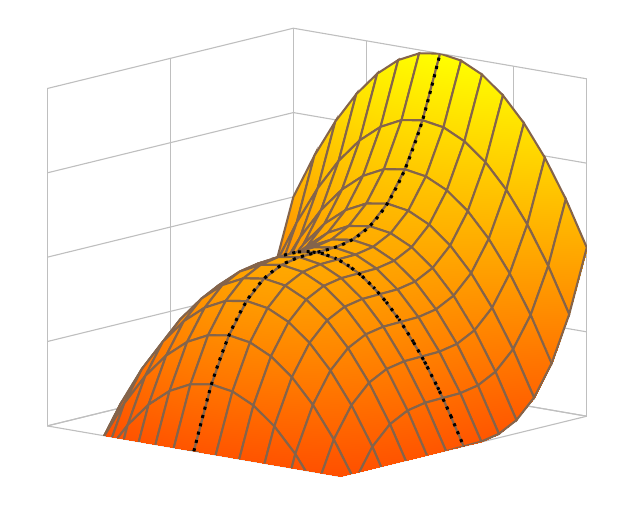
\begin{tikzpicture}
\begin{axis}[xmin=-1.0,xmax=1.0,
             ymin=-1.0,ymax=1.0,
             zmin=-1.0,zmax=1.0,
             grid=major,
             axis line style={draw=none},
             tick style={draw=none},
             view={310}{35},
             xticklabels={\empty},
             yticklabels={\empty},
             zticklabels={\empty},
             plot box ratio={1 1 3},
             colormap/redyellow]
\newcommand\func[2]{#1^3 - #2^2}
\definecolor{darkorange}{HTML}{84644B}

    \addplot3[surf,
              shader=faceted interp,
              faceted color={darkorange},
              samples=15,
              domain=-1:1,
              y domain=-1:1] {\func{x}{y}};

    % plot curve for x direction
    \addplot3[samples=15,
              domain=-1:1,
              samples y=1,
              dotted,
              black,
              line width=1.1pt,
              smooth] (x, 0, \func{x}{0});
    % plot curve for y direction
    \addplot3[samples=15,
              domain=-1:1,
              y domain=-1:0.22,
              dotted,
              black,
              line width=1.1pt,
              smooth] (0, y, \func{0}{y});
\end{axis}
\end{tikzpicture}

        }
        \caption{The curvature of a surface at a given point depends on the direction of measurement. The principal curvatures are the maximum and minimum value of curvatures in all directions.}
    \end{subfigure}
\end{figure}

As a different analytical approach to producing feature images the calculation of the \gls{curvature} for each depth value.
The two common measures of curvature in differential geometry are \gls{gaussian-curvature} and \gls{mean-curvature}\cite{Kuhnel2008}.

If the function is known as a graph the \Gls{gaussian-curvature} can be estimated using the derivatives of the function.
For depth data each depth value is a sample of this function graph and numeric approximation of the derivatives allows the calculation of the curvature.
\begin{align}
    \mathfrak{K} &= \frac{f_{uu} f_{vv} - f_{uv}^2}{{(1 + f_u^2 + f_v^2)}^2}
\end{align}
With
\begin{align*}
    f_{x} &= \frac{y_1 - y_0}{\Delta x} \\
    f_{xx} &= \frac{y_1 + y_{-1} - 2 y_0}{{\Delta x}^2}
\end{align*}
as approximation for the derivatives.

Similarly, the \Gls{mean-curvature} can be calculated with a different formula.
\begin{align}
    \mathfrak{H} &= \frac{{(1 + f_{v}^2)} f_{uu} - 2 f_u f_v f_{uv} + {(1 + f_u^2)} f_{vv}}{2 \sqrt{1 + f_u^2 + f_v^2}^3}
\end{align}
Both measures of curvature are $\mathfrak{K},\mathfrak{H} \in {\rm I\!R}$.
To convert them into a meaningful grayscale image they need to be clamped to arbitrary bounds, that can be choosen based on visual distinctiveness or other heuristics.
After clamping the values are scaled and quantized accordingly.

\subsubsection{Multi-Directional Bearing Angle}

The \gls{max-curve-image} tries generalize the \gls{bearing-angle} to be rotation invariant as it takes the \gls{bearing-angle} in each direction into account.
Additionally to the left-sided \gls{bearing-angle} the right-sided angle is calculated as well and finally added.

\begin{figure}
    

\tikzset{every picture/.style={line width=0.75pt}} %set default line width to 0.75pt        

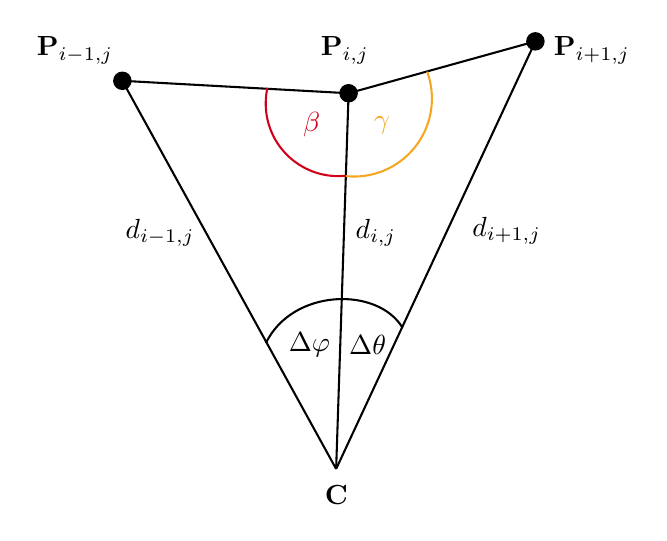
\begin{tikzpicture}[x=0.75pt,y=0.75pt,yscale=-1,xscale=1]
%uncomment if require: \path (0,252); %set diagram left start at 0, and has height of 252

%Straight Lines [id:da05017383740499093] 
\draw    (46.83,26.67) -- (149.83,213.67) ;
%Straight Lines [id:da6895513561877372] 
\draw    (155.83,32.67) -- (149.83,213.67) ;
%Curve Lines [id:da10253757735662583] 
\draw [color={rgb, 255:red, 0; green, 0; blue, 0 }  ,draw opacity=1 ]   (116,153) .. controls (128.83,126.67) and (169.83,125.67) .. (181.83,145.67) ;
%Straight Lines [id:da3851492122035306] 
\draw    (46.83,26.67) -- (155.83,32.67) ;
%Shape: Circle [id:dp08101382020617043] 
\draw  [fill={rgb, 255:red, 0; green, 0; blue, 0 }  ,fill opacity=1 ] (151.88,32.67) .. controls (151.88,30.49) and (153.65,28.72) .. (155.83,28.72) .. controls (158.01,28.72) and (159.78,30.49) .. (159.78,32.67) .. controls (159.78,34.85) and (158.01,36.62) .. (155.83,36.62) .. controls (153.65,36.62) and (151.88,34.85) .. (151.88,32.67) -- cycle ;
%Shape: Circle [id:dp7397482298206297] 
\draw  [fill={rgb, 255:red, 0; green, 0; blue, 0 }  ,fill opacity=1 ] (42.88,26.67) .. controls (42.88,24.49) and (44.65,22.72) .. (46.83,22.72) .. controls (49.01,22.72) and (50.78,24.49) .. (50.78,26.67) .. controls (50.78,28.85) and (49.01,30.62) .. (46.83,30.62) .. controls (44.65,30.62) and (42.88,28.85) .. (42.88,26.67) -- cycle ;
%Shape: Circle [id:dp7936487176657823] 
\draw  [fill={rgb, 255:red, 0; green, 0; blue, 0 }  ,fill opacity=1 ] (241.88,7.67) .. controls (241.88,5.49) and (243.65,3.72) .. (245.83,3.72) .. controls (248.01,3.72) and (249.78,5.49) .. (249.78,7.67) .. controls (249.78,9.85) and (248.01,11.62) .. (245.83,11.62) .. controls (243.65,11.62) and (241.88,9.85) .. (241.88,7.67) -- cycle ;
%Straight Lines [id:da7225304487809803] 
\draw    (245.83,7.67) -- (149.83,213.67) ;
%Straight Lines [id:da15289701870660388] 
\draw    (155.83,32.67) -- (245.83,7.67) ;
%Shape: Arc [id:dp845909277560968] 
\draw  [draw opacity=0] (154.29,72.43) .. controls (153.16,72.54) and (152.02,72.6) .. (150.87,72.6) .. controls (131.56,72.6) and (115.9,56.94) .. (115.9,37.63) .. controls (115.9,35.08) and (116.17,32.59) .. (116.69,30.19) -- (150.87,37.63) -- cycle ; \draw  [color={rgb, 255:red, 208; green, 2; blue, 27 }  ,draw opacity=1 ] (154.29,72.43) .. controls (153.16,72.54) and (152.02,72.6) .. (150.87,72.6) .. controls (131.56,72.6) and (115.9,56.94) .. (115.9,37.63) .. controls (115.9,35.08) and (116.17,32.59) .. (116.69,30.19) ;
%Shape: Arc [id:dp15343497156889918] 
\draw  [draw opacity=0] (193.67,22.29) .. controls (195.16,26.33) and (195.97,30.7) .. (195.97,35.25) .. controls (195.97,55.99) and (179.15,72.8) .. (158.42,72.8) .. controls (157.06,72.8) and (155.72,72.73) .. (154.4,72.59) -- (158.42,35.25) -- cycle ; \draw  [color={rgb, 255:red, 245; green, 166; blue, 35 }  ,draw opacity=1 ] (193.67,22.29) .. controls (195.16,26.33) and (195.97,30.7) .. (195.97,35.25) .. controls (195.97,55.99) and (179.15,72.8) .. (158.42,72.8) .. controls (157.06,72.8) and (155.72,72.73) .. (154.4,72.59) ;

% Text Node
\draw (137,154) node  [color={rgb, 255:red, 0; green, 0; blue, 0 }  ,opacity=1 ] [align=left] {$\displaystyle \Delta $$\displaystyle \varphi $};
% Text Node
\draw (138,48) node  [color={rgb, 255:red, 208; green, 2; blue, 27 }  ,opacity=1 ] [align=left] {$\displaystyle \beta $};
% Text Node
\draw (169,100) node   [align=left] {$\displaystyle d_{i,j}$};
% Text Node
\draw (65,100) node   [align=left] {$\displaystyle d_{i-1,j}$};
% Text Node
\draw (154,12) node   [align=left] {$\displaystyle \mathbf{P}_{i,j}$};
% Text Node
\draw (150,226) node   [align=left] {$\displaystyle \mathbf{C}$};
% Text Node
\draw (232,99) node   [align=left] {$\displaystyle d_{i+1,j}$};
% Text Node
\draw (172,48) node   [align=left] {$\displaystyle \textcolor[rgb]{0.96,0.65,0.14}{\gamma }$};
% Text Node
\draw (165,154) node  [color={rgb, 255:red, 0; green, 0; blue, 0 }  ,opacity=1 ] [align=left] {$\displaystyle \Delta $$\displaystyle \theta $};
% Text Node
\draw (273,12) node   [align=left] {$\displaystyle \mathbf{P}_{i+1,j}$};
% Text Node
\draw (24,12) node   [align=left] {$\displaystyle \mathbf{P}_{i-1,j}$};


\end{tikzpicture}


    \caption[Schematic Representation of the Max-Curve]{The Max-Curve composes two \Glspl{bearing-angle} in vertical, horizontal, diagonal and antidiagonal direction. The maximum angle is then selected as pixel value.}
\end{figure}

This makes the measure more robust to rotation, but does not produce good features.
\begin{align}
    B &= \max{\{B_{diagonal}, B_{antidiagonal}, B_{horizontal}, B_{vertical}\}}
\end{align}

\subsubsection{Viability of Conversions}

\begin{itemize}
    \item effect of noisy input
    \item soundness and mathematical foundation
    \item computational complexity
    \item Discussion of characteristic for Bearing Flexion.
\end{itemize}

\subsubsection{Implementation Notes}

Formulas pictures and short computational evaluation.
Each implementation is independent of the camera model.
Describe the concepts required for implementation.
Both serial and parallel execution.
Parallel execution is done row-wise over all cores using CppTaskflow based Task Scheduling.
No explicit use SIMD, because OpenCV\cite{opencv_library} is used for data storing proper memory alignment is already ensured.
Specialized optimiziation should allow the use of SIMD with OpenCV's Hardware Abstraction Layer.

Focus on correctness and generality.
Provided implementation should rather serve as reference implementation that can be used to validate optimized implementations.

\begin{lstlisting}
template <template <typename> typename Intrinsic,
          typename Real>
inline constexpr bool is_intrinsic_v =
  std::is_floating_point_v<Real>
  &&
  std::is_same_v<typename Intrinsic<Real>::real_type, Real>
  &&
  std::is_invocable_r_v<
    int,
    decltype(&Intrinsic<Real>::w),
    Intrinsic<Real>
  >
  &&
  std::is_invocable_r_v<
    int,
    decltype(&Intrinsic<Real>::h),
    Intrinsic<Real>
  >
  &&
  std::is_invocable_r_v<
    math::sphere_coord<Real>,
    decltype(&Intrinsic<Real>::template pixel_to_sphere<int>),
    Intrinsic<Real>,
    math::pixel_coord<int>
  >
  &&
  std::is_invocable_r_v<
    math::sphere_coord<Real>,
    decltype(&Intrinsic<Real>::template pixel_to_sphere<Real>),
    Intrinsic<Real>,
    math::pixel_coord<Real>
  >
  &&
  std::is_invocable_r_v<
    math::pixel_coord<Real>,
    decltype(&Intrinsic<Real>::template camera_to_pixel<Real>),
    Intrinsic<Real>,
    math::camera_coord<Real>
  >
  &&
  std::is_invocable_r_v<
    math::pixel_coord<int>,
    decltype(&Intrinsic<Real>::template camera_to_pixel<int>),
    Intrinsic<Real>,
    math::camera_coord<Real>
  >;
\end{lstlisting}

